\section{Struktur der Proben}

Alle in diesem Versuch untersuchten Materialien (Gold,Graphit und eine unbekannte Probe) sind Leiter, sie unterscheiden sich jedoch in der Konfiguration der Elektronen. Es gibt einen unterschied zwischen der Verteilung der Elektronen in Metallen und Halbleitern. Metalle werde dabei durch das Elektronen-Gas beschrieben und somit eine homogen Verteilung angenommen wird. Bei der Beschreibung von Halbleitern m�ssen noch Bandl�cken ber�cksichtigt werden. Da die r�umliche Verteilung der Elektronen nicht homogen ist, kann aus der Ladungsverteilung die Position der Atome bestimmt werden. Es soll nun genauer auf die beiden bekannten Proben Gold und Graphit eingegangen werden.

\subsection{Graphit}

Die Graphitporbe ist ein HOPG (Highly orderd pyrolytic graphit), ein Halbleiter mit einer hcp-Gitterstruktur. In Abbildung ?? ist die Gitterstruktur des Graphit zu sehen. In einer Ebene werden die Kohlenstoffatome aufgrund der sp2-Hybirdisirung  stark durch kovalente Bindungen zusammengehalten. Zwischen den Ebenen werde die Kohlenstoffatome nur von Van-der-Waals-Kr�ften zusammengehalten. 

\begin{figure}[H]
	\centering
  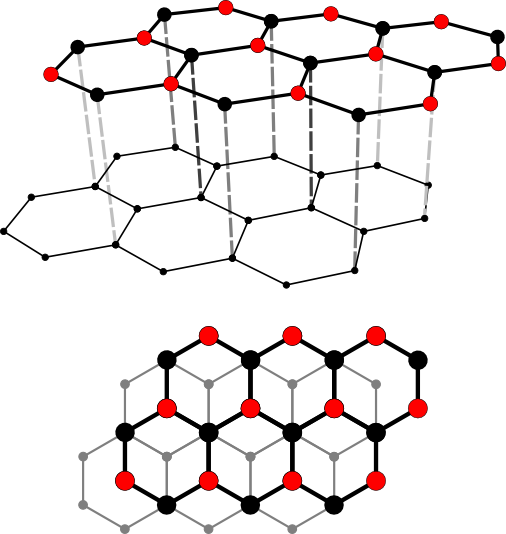
\includegraphics[scale=0.8]{graphit.png}
	\caption{Schematische Struktur von Graphit. Es liegen immer die 2n und die 2n-1 Ebene genau �bereinander. Die Ebenen untereinander besitzen nur an jedem zweitem Punkt der Hexagonale eine Verbindung. Entnommen von ??}
	\label{fig:graphit}
\end{figure}